%=-=-=-=-=-=-=-=-=-=-=-=-=-=-=-=-=-=-=-=-=-=-=-=-=-=-=-=-=-=-=-=-=-=- CHAPTER 01
\chapter{images}

%=-=-=-=-=-=-=-=-=-=-=-=-=-=-=-=-=-=-=-=-=-=-=-=-=-=-=-=-=-=-=-=-=-=-=-= SECTION
\section{Storing Images}
It would probabily be best if you stored all of your images in a dedicated folder.
I like to keep my images in a folder called \verb!assets!.  


%=-=-=-=-=-=-=-=-=-=-=-=-=-=-=-=-=-=-=-=-=-=-=-=-=-=-=-=-=-=-=-=-=-=-=-= SECTION
\section{Figure}

All images should be included within a figure environment.

\begin{figure}[h]
    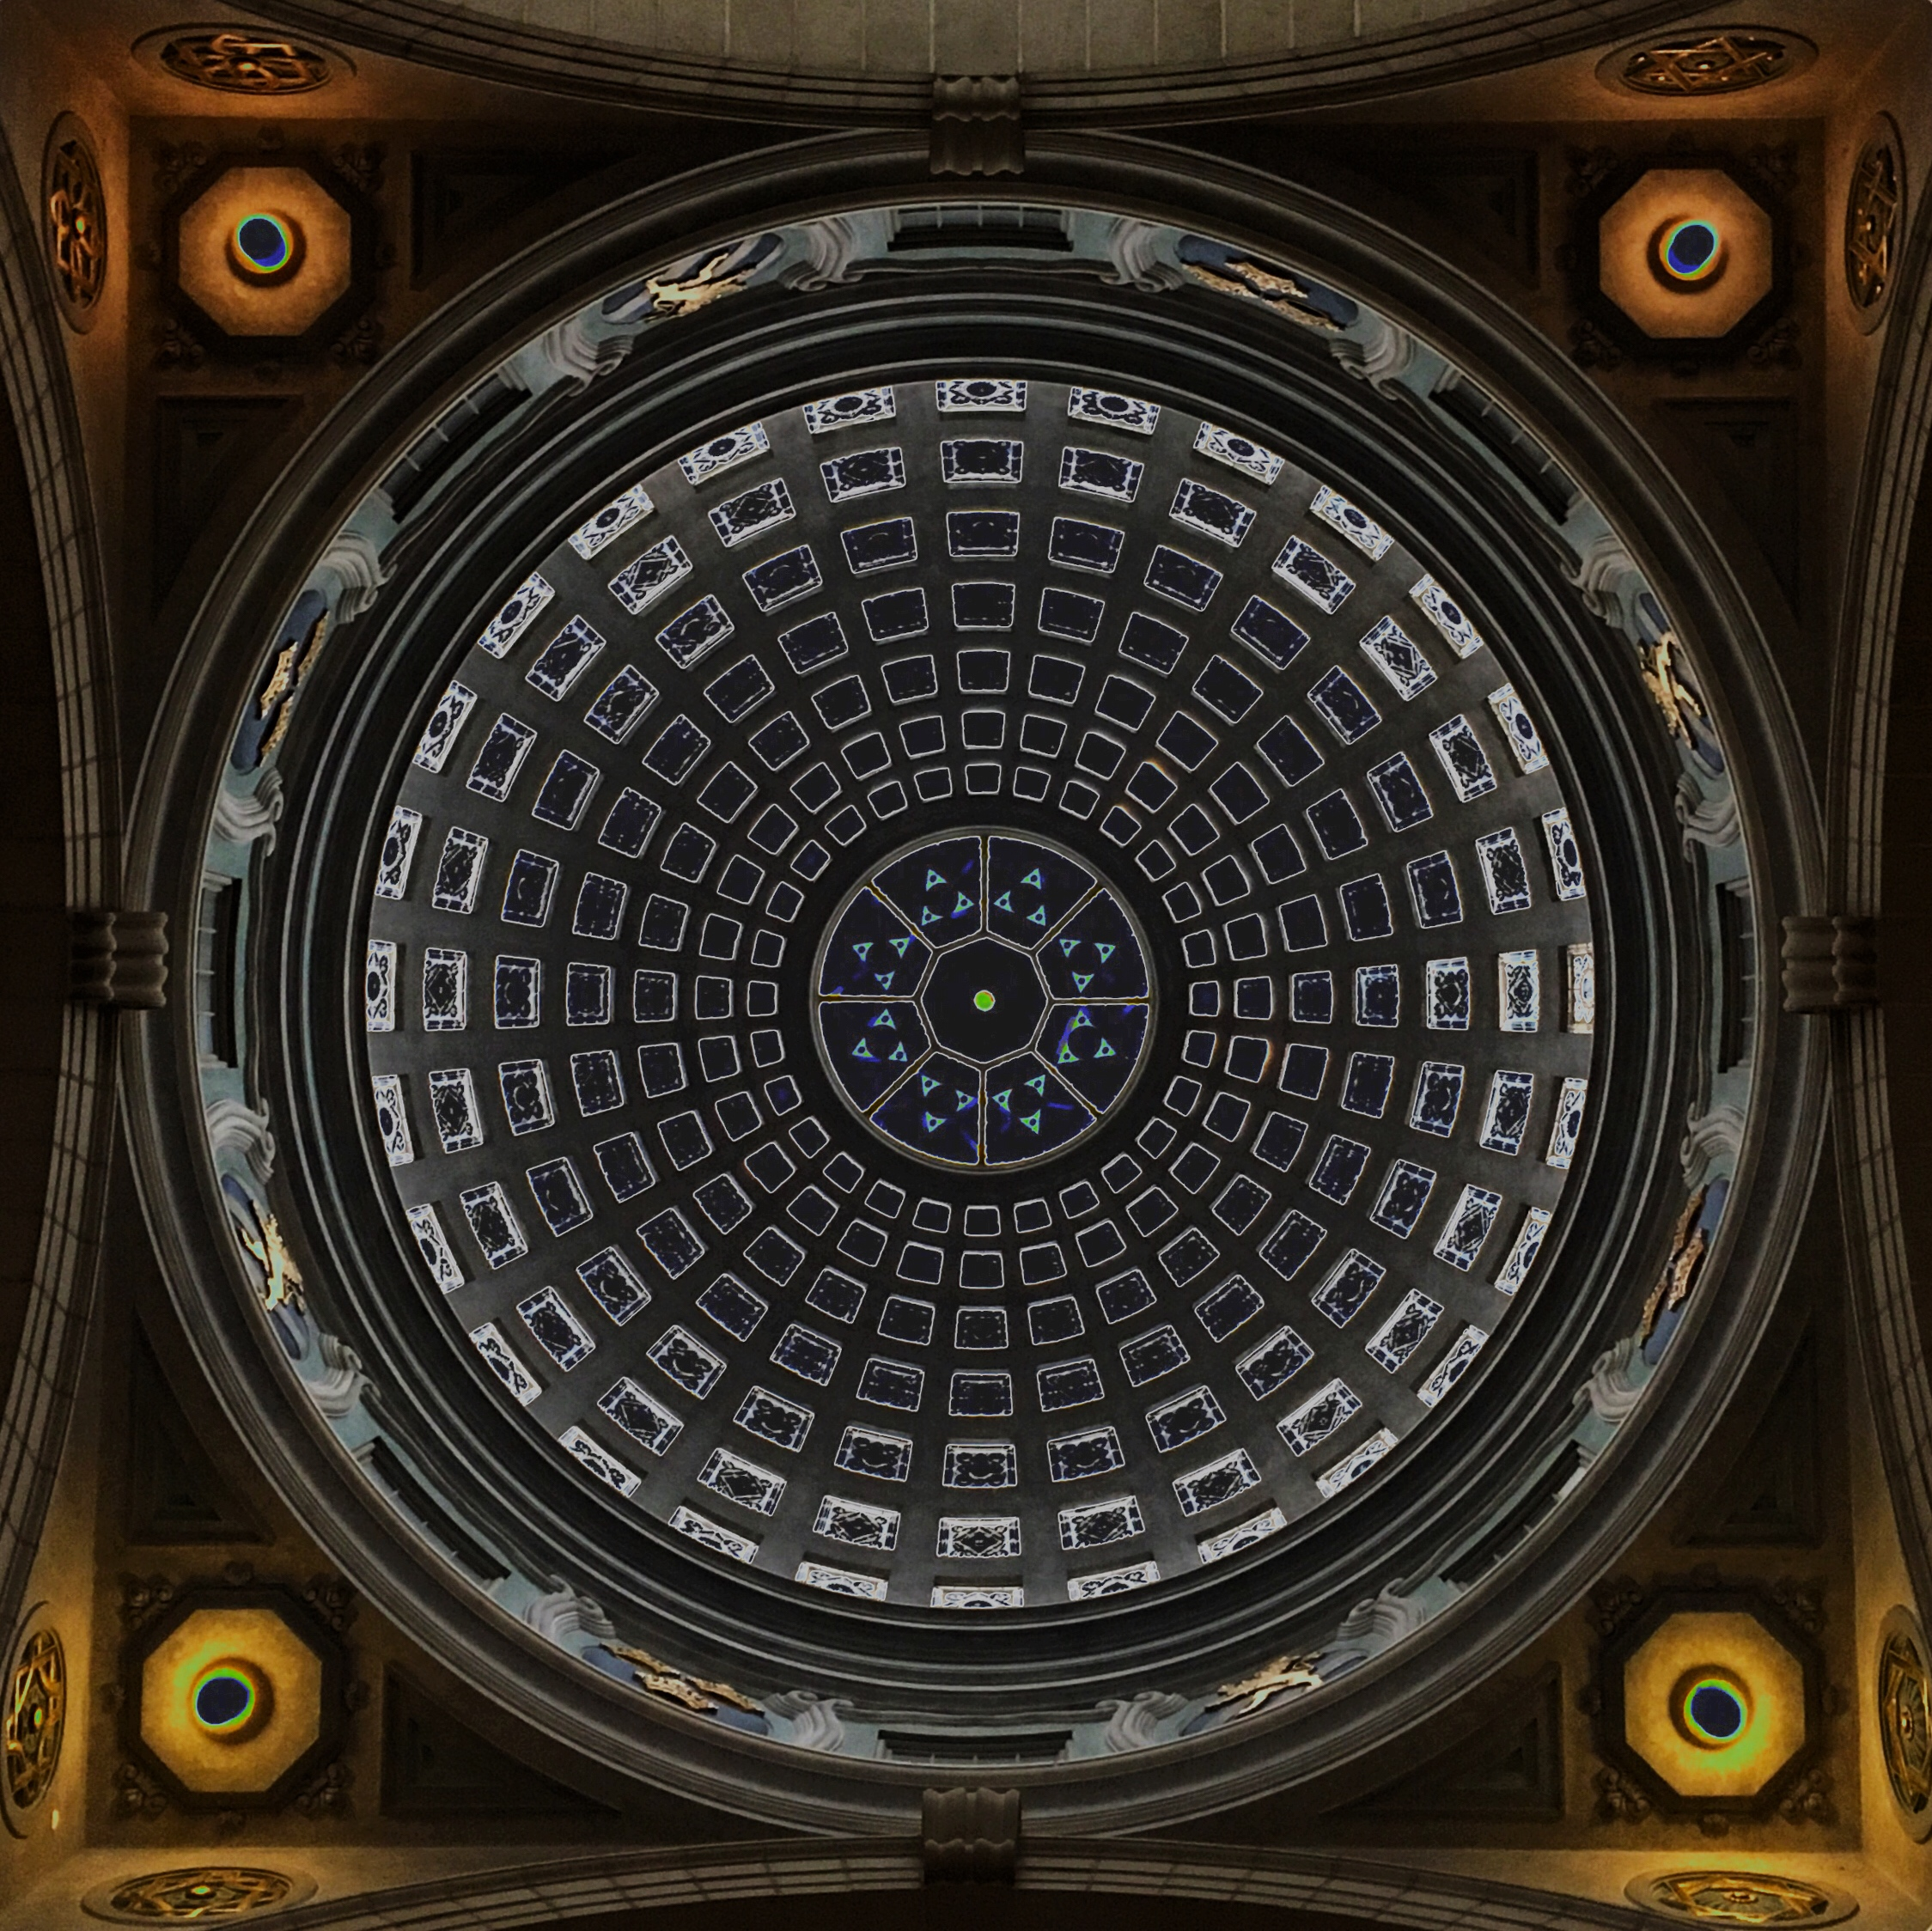
\includegraphics[width = 0.5\textwidth]{assets/image.jpg}
    \caption{Here is my excellent image.}
    \label{fig:img001}
\end{figure}

Notice how easy it is for me to reference the above as figure \ref{fig:img001}.

It is also possible to include multiple images that are horizontally aligned.

\begin{figure}
    \centering
    \begin{subfigure}[b]{0.3\textwidth}
        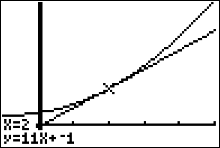
\includegraphics[width=\textwidth]{./assets/20170509-123642}
        \caption{Step 1}
        \label{fig:step1}
    \end{subfigure}
    ~ %add desired spacing between images, e. g. ~, \quad, \qquad, \hfill etc. 
      %(or a blank line to force the subfigure onto a new line)
    \begin{subfigure}[b]{0.3\textwidth}
        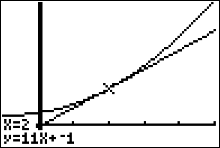
\includegraphics[width=\textwidth]{./assets/20170509-123642.png}
        \caption{Step 2}
        \label{fig:step2}
    \end{subfigure}
    ~ %add desired spacing between images, e. g. ~, \quad, \qquad, \hfill etc. 
    %(or a blank line to force the subfigure onto a new line)
    \begin{subfigure}[b]{0.3\textwidth}
        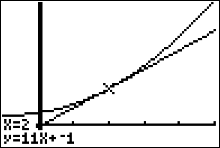
\includegraphics[width=\textwidth]{./assets/20170509-123642.png}
        \caption{Step 3}
        \label{fig:step3}
    \end{subfigure}
    \caption{The Steps Shown}\label{fig:threesteps}
\end{figure}